
%\documentclass[a4paper]{article}
%
%\author{Rasmus Tibell}
%\title{Master Thesis Example}
%
%\usepackage{graphicx}
%\usepackage{multirow}
%\usepackage{mathtools}
%\begin{document}


%\section{The mathematics behind the Multi\-layer Perseptron}
The model consists of L feature variables, this is the same number as input neurons, figure  \ref{NeuralNet_InHidHidOut} shows the configuration of the network.
Each record in the training data is comprised of the feature variables $\textbf{x} =\{x_{(1)}, x_{(2)}, \ldots , x_{(L)}\}$
 and a target variable y. The training set consists of M tuples as follows: 
 $\textbf{T} =\{(x^{(1)}, y^{(1)}), (x^{(2)}, y^{(2)}), \ldots , (x^{(M)}, y^{(M)})\}$


\subsection{Layout of the neural netowork}
This paper will mainly cover multilayer perseptrons with input nodes, one or two hidden layers and a regression output node. Note that only regression output will be used so the output unit is linear and no Softmax will be included. 

\begin{figure}[h!] 
\begin{center}
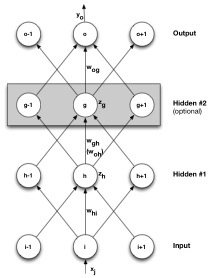
\includegraphics{NeuralNet_InHidOut.jpg}
\caption{Layout of \textit{neural network}. Note that the hidden layer in the lower part of the figure are optional, both network with one and two hidden layers will be discussed.}
\label{NeuralNet_InHidHidOut}
\end{center}
\end{figure}

Let I denote the number of output neurons and H,G the number of hidden units, see figure \ref{NeuralNet_InHidHidOut}. Finaly the number of input neurons are given by L.


\subsection{Error function}
The error function is used to measure the error between the actual value and the prediction. Define the error function E (equation \ref{eq:error_function}) as the sum of the squared differances between the expected and calculated output , $n \in trainingset$. Nota bene that the erorr function for the regression case is different from the functioin used with classification.
\begin{equation} \label{eq:error_function}
E = \frac{1}{2} \sum_{n}{(t^{(n)}-y^{(n)})^{2}}
\end{equation}

Taking the derivative of E (equation \ref{eq:error_function}) with respect to the weights gives us the following function:

\begin{equation} \label{eq:error_function_part_w} 
\frac{\partial{E}}{\partial{w_{i}}} = \frac{1}{2} \sum_{n}{\frac{\partial{y^{(n)}}}{\partial{w_{i}}} \frac{\partial{E}}{\partial{y^{(n)}}}} = -\sum_{n}{\frac{\partial{y^{(n)}}}{\partial{w_{i}}}(t^{(n)}-y^{(n)})}
\end{equation}
\\
We can now form the batch delta rule $\Delta w_{i}$ as
\begin{equation} \label{eq:batch_delta_rule}
\Delta w_{i} = -\epsilon \frac{\partial{E}}{\partial{w_{i}}} = \sum_{n}{\epsilon \frac{\partial{y^{(n)}}}{\partial{w_{i}}}(t^{(n)}-y^{(n)})}
\end{equation}




\subsection{Activation functions in the nodes}
ToDo
\subsubsection{Output neuron (Linear)}
The linear neurons activation function is defined as
\begin{equation} \label{eq:linj_func}
y = \sum_{i}x_{i}w_{i} 
\end{equation} 
\\
The partial derivatives of the linear activation function are
\begin{equation} \label{eq:linear_partial_w}
\frac{\partial{y}}{\partial{w_{i}}} = x_{i}
\end{equation}
and
\begin{equation} \label{eq:linear_partial_x}
\frac{\partial{y}}{\partial{x_{i}}} = w_{i}
\end{equation}

\subsubsection{Logistic neuron (Sigmoid)}
Define the activation function for the logistic neuron as
\begin{equation} \label{eq:sigmoid_func}
y = \frac{1}{1+e^{-z}} 
\end{equation}  
where 
\begin{equation} \label{eq:sigmoid_func_z}
 z = b+\sum_{i}x_{i}w_{i}
\end{equation}  
\\
The derivative of y is $\frac{dy}{dz} = y(1-y)$
\\
Partial derivatives for z are $\frac{\partial{z}}{\partial{w_{i}}} = x_{i}$ and $\frac{\partial{z}}{\partial{x_{i}}} = w_{i}$. Now can the partial derivative of y with respect to $w_{i}$ be defined
\begin{equation} \label{eq:sigmoid_partial_w}
\frac{\partial{y}}{\partial{w_{i}}} =\frac{\partial{y}}{\partial{z}}\frac{\partial{z}}{\partial{w_{i}}} = y(1-y)x_{i}
\end{equation}

\subsubsection{Hyperbolig tangent neuron}
Hyperbolic neuron is defined as
\begin{equation} \label{eq:tanh_func}
y = \frac{e^{z}-e^{-z}}{e^{z}+e^{-z}}
\end{equation}
where 
\begin{equation} \label{eq:tanh_func_z}
z = b+\sum_{i}x_{i}w_{i} 
\end{equation} 
\\
The derivative of y is $\frac{dy}{dz} = (1+y)(1-y)$
\\
Partial derivatives for z are $\frac{\partial{z}}{\partial{w_{i}}} = x_{i}$ and $\frac{\partial{z}}{\partial{x_{i}}} = w_{i}$. From this follows the partial derivative of y with respect to $w_{i}$ is
\begin{equation} \label{eq:tanh_partial_w}
\frac{\partial{y}}{\partial{w_{i}}} =\frac{\partial{y}}{\partial{z}}\frac{\partial{z}}{\partial{w_{i}}} = (1+y)(1-y)x_{i}
\end{equation}
and that the partial derivative of y with respect to $x_{i}$ is
\begin{equation} \label{eq:tanh_partial_x}
\frac{\partial{y}}{\partial{x_{i}}} =\frac{\partial{y}}{\partial{z}}\frac{\partial{z}}{\partial{x_{i}}} = (1+y)(1-y)w_{i}
\end{equation}


\subsection{Finding the gradiants for the error function}
In this section the gradient for the error function both for multilayer perceptrons with singe and dual layers of hidden units is defined. The notations is based on the network configuration shown in figure \ref{NeuralNet_InHidHidOut}.

\subsubsection{Single hidden layer with hyperbolic activation function} \label{ch:single_hidden_layer}
We need to find $\frac{\partial{E}}{\partial{w_{oh}}}$ and $\frac{\partial{E}}{\partial{w_{hi}}}$ in order to performe the calcualtions required by the back propagation algorithm. As before $\epsilon$ is the lerning of the gradient decent. We use $\Delta w_{oh}$ and $\Delta w_{hi} $ to update the wights $w_{oh}$ and $w_{hi}$ respectivly. 
N is the number of observations in a minibatch and $n \in minibatch$.

For the first weight between the output node and the hidden unit we need to calculate $\Delta w_{oh}$.

\begin{equation} \label{eq:gen_error_d_weight_oh}
\Delta w_{oh} = \epsilon \frac{\partial{E}}{\partial{w_{oh}}} = \epsilon \frac{\partial{E}}{\partial{y^{(n)}_{o}}} \frac{\partial{y^{(n)}_{o}}}{\partial{w_{oh}}}
\end{equation}

From equation (\ref{eq:error_function_part_w}) we get $\frac{\partial{E}}{\partial{y}}$
and from equation (\ref{eq:linear_partial_w}) we get $\frac{\partial{y}}{\partial{w_{oh}}}$.
This gives us the solution for equation (\ref{eq:gen_error_d_weight_oh}) as
\begin{equation} \label{eq:gen_error_d_weight_oh_final}
\Delta w_{oh}  = \epsilon \sum_{n} (t^{(n)_{o}}-y^{(n)}_{o}) z^{(n)}_{h} 
\end{equation}

The delta for the weigths between the input node and the hidden layer is given by $\Delta w_{hi} $. 

\begin{equation} \label{eq:gen_error_d_weight_hi}
\Delta w_{hi} = \epsilon \frac{\partial{E}}{\partial{w_{hi}}} = \epsilon \frac{\partial{E}}{\partial{y^{(n)}_{o}}} \frac{\partial{y^{(n)}_{o}}}{\partial{z^{(n)}_{h}}} \frac{\partial{z^{(n)}_{h}}}{\partial{w_{hi}}}
\end{equation}
From equation (\ref{eq:error_function_part_w}) we get $\frac{\partial{E}}{\partial{y}}$
and from equation (\ref{eq:linear_partial_x}) we get $\frac{\partial{y}}{\partial{z_{h}}}$.
The final part $\frac{\partial{z_{h}}}{\partial{w_{hi}}}$ can we obtain from equation (\ref{eq:tanh_partial_w}). This gives us sulution for equation (\ref{eq:gen_error_d_weight_hi}) as
\begin{multline} \label{eq:gen_error_d_weight_hi_final}
\Delta w_{hi}  = \epsilon \frac{\partial{E}}{\partial{y^{(n)}_{o}}} \frac{\partial{y^{(n)}_{o}}}{\partial{z^{(n)}_{h}}} \frac{\partial{z^{(n)}_{h}}}{\partial{w_{hi}}} = \\
\epsilon \sum_{n} \sum_{o}(t^{(n)}_{o}-y^{(n)}_{o}) w_{oh} (1+z^{(n)}_{h})(1-z^{(n)}_{h}) x^{(n)}_{i}
\end{multline}




\subsubsection{Dual hidden layers with hyperbolic activation function} \label{ch:dual_hidden_layer}
For the dual hidden layer configuration we are going to use the two delta wights $\frac{\partial{E}}{\partial{w_{og}}}$ (previously named $\frac{\partial{E}}{\partial{w_{oh}}}$) and $\frac{\partial{E}}{\partial{w_{gh}}}$ (previously named $\frac{\partial{E}}{\partial{w_{hi}}}$) from previous section \ref{ch:single_hidden_layer} and one aditional weight between the input nodes and lower hidden layer $\frac{\partial{E}}{\partial{w_{hi}}}$, for the notations see figure \ref{NeuralNet_InHidHidOut}.
\\
The delta for the weights between the output units and the upper hidden layer, $\Delta w_{og}$ is given by equation ($\ref{eq:gen_error_d_weight_oh}$) but with the indexes renamed. 
\begin{equation} \label{eq:gen_dual_error_d_weight_og}
\Delta w_{og} = 
\epsilon \frac{\partial{E}}{\partial{w_{og}}} = 
\epsilon \frac{\partial{E}}{\partial{y^{(n)}_{o}}} \frac{\partial{y^{(n)}_{o}}}{\partial{w_{og}}} = 
\epsilon \sum_{n} (t^{(n)}_{o}-y^{(n)}_{o}) z^{(n)}_{g}
\end{equation}


The same holds for the delta weights between the two hidden layers $\Delta w_{gh}$ that can be obtained by rewriting the indexes of equation ($\ref{eq:gen_error_d_weight_hi}$) with the indexes renamed. 

\begin{multline} \label{eq:gen_dual_error_d_weight_gh}
\Delta w_{gh} = 
\epsilon \frac{\partial{E}}{\partial{w_{gh}}} = 
\epsilon \frac{\partial{E}}{\partial{y^{(n)}_{o}}} \frac{\partial{y^{(n)}_{o}}}{\partial{z^{(n)}_{g}}} \frac{\partial{z^{(n)}_{g}}}{\partial{w_{gh}}} = \\
\epsilon \sum_{n} \sum_{o}(t^{(n)}_{o}-y^{(n)}_{o}) w_{og} (1+z^{(n)}_{g})(1-z^{(n)}_{g}) z^{(n)}_{h}
\end{multline}

For the final delta weight  $\Delta w_{hi}$ we have to perform some additional work to solve the equation. We need to find the partial derivative $\frac{\partial{z^{(n)}_{g}}}{\partial{z^{(n)}_{h}}}$. Using the equation ($\ref{eq:tanh_partial_x}$) we can get
\begin{displaymath}
\frac{\partial{z^{(n)}_{g}}}{\partial{z^{(n)}_{h}}} = (1+z^{(n)}_{g})(1-z^{(n)}_{g}) w_{gh}
\end{displaymath}

Now we can find the equation for $\Delta w_{hi}$ using the above partial derivative
\begin{multline} \label{eq:gen_dual_error_d_weight_hi_final}
\Delta w_{hi}  = 
\epsilon \frac{\partial{E}}{\partial{w_{hi}}} = 
\epsilon \frac{\partial{E}}{\partial{y^{(n)}_{o}}} \frac{\partial{y^{(n)}_{o}}}{\partial{z^{(n)}_{g}}} \frac{\partial{z^{(n)}_{g}}}{\partial{z^{(n)}_{h}}} \frac{\partial{z^{(n)}_{h}}}{\partial{w_{hi}}} = \\
\epsilon \sum_{n} \sum_{o} \sum_{g} (t^{(n)}_{o}-y^{(n)}_{o}) w_{og} (1+z^{(n)}_{g})(1-z^{(n)}_{g}) w_{gh} (1+z^{(n)}_{h})(1-z^{(n)}_{h}) x^{(n)}_{i}
\end{multline}





\subsection{Matrix calculations for the MLP}
Let $H_{1}$ and $H_{2}$ be the number of hidden units for layer 1 and 2. The number of inputs are represented by $I$ and the number of observation in a minibatch is $N$. For regression output, as in this paper the number of output units is equal to one and is denoted by $O$.  

Let $\mathbf{X}$ be a $I \times N$ matrix of the input features in a minibatch, $\mathbf{Y}$ and $\mathbf{T}$ are matrices of size $O \times N$ and denotes the predicted value and target value respectively. 

\subsubsection{Single hidden layer with hyperbolic activation function} \label{ch:mtx_single_hidden_layer}
 Let $\mathbf{\Theta}$ be the $O \times H_{1}$ matrix of weights on the connection from hidden units to output units and $\mathbf{W}$ is the $I \times H_{1}$ matrix with weights on the connections from input units to the hidden units. The output of the hidden unit is represented as a $H_{1} \times N$ matrix $\mathbf{\Psi}$ for a single minibatch.  
 \\
 Now we can represent the equation (\ref{eq:gen_error_d_weight_oh_final}) in vectorized form as
\begin{displaymath}
 \frac{1}{N}(\mathbf{Y}-\mathbf{T}) \mathbf{\Psi^{T}} 
 \end{displaymath}
 \\
 and for equation (\ref{eq:gen_error_d_weight_hi_final}) we get
 \begin{displaymath}
 \frac{1}{N}(\mathbf{\Theta^{T}}(\mathbf{Y}-\mathbf{T})) \circ (\mathbf{1} - \mathbf{\Psi}) \circ (\mathbf{1} - \mathbf{\Psi}) \mathbf{X^{T}}
 \end{displaymath}

\subsubsection{Dual hidden layers with hyperbolic activation function} \label{ch:mtx_dual_hidden_layer}
Now let $\mathbf{\Theta}$ be the $O \times H_{2}$ matrix of weights on the connection from the second layer of hidden units to output units and $\mathbf{W}$ is the $I \times H_{1}$ matrix with weights on the connections from input units to the first layer of hidden units. The output of the first hidden unit is represented as a $H_{1} \times N$ matrix $\mathbf{\Upsilon}$ and a $H_{2} \times N$ matrix $\mathbf{\Psi}$ for the second layer.
Let $\mathbf{\Xi}$ be the $H_{1} \times H_{2}$ matrix of weights on the connections between the hidden layers.
\\
 Now we can represent the equation (\ref{eq:gen_dual_error_d_weight_og}) in vectorized form as
\begin{displaymath}
 \frac{1}{N}(\mathbf{Y}-\mathbf{T}) \mathbf{\Psi^{T}} 
 \end{displaymath}
 \\
 and for equation (\ref{eq:gen_dual_error_d_weight_gh}) we get
 \begin{displaymath}
 \frac{1}{N}(\mathbf{\Theta^{T}}(\mathbf{Y}-\mathbf{T})) \circ (\mathbf{1} - \mathbf{\Psi}) \circ (\mathbf{1} - \mathbf{\Psi}) \mathbf{\Upsilon^{T}}
 \end{displaymath}
  and finaly for equation (\ref{eq:gen_dual_error_d_weight_hi_final}) we get
\begin{displaymath}
 \frac{1}{N}\Xi((\mathbf{\Theta^{T}}(\mathbf{Y}-\mathbf{T})) \circ (\mathbf{1} - \mathbf{\Psi}) \circ (\mathbf{1} + \mathbf{\Psi})) \circ
 (\mathbf{1} - \mathbf{\Upsilon}) \circ (\mathbf{1} + \mathbf{\Upsilon}) \mathbf{X^{T}}
 \end{displaymath}

If we take the weight decay into account the final matrix representation for equations (\ref{eq:gen_dual_error_d_weight_og}, \ref{eq:gen_dual_error_d_weight_gh}, \ref{eq:gen_dual_error_d_weight_hi_final}) becomes
\begin{displaymath}
\frac{1}{N}(\mathbf{Y}-\mathbf{T}) \mathbf{\Psi^{T}} + \lambda \Theta
 \end{displaymath}
 \begin{displaymath}
 \frac{1}{N}(\mathbf{\Theta^{T}}(\mathbf{Y}-\mathbf{T})) \circ (\mathbf{1} - \mathbf{\Psi}) \circ (\mathbf{1} - \mathbf{\Psi}) \mathbf{\Upsilon^{T}} + \lambda \Xi
\end{displaymath}
\begin{displaymath}
\frac{1}{N}\Xi((\mathbf{\Theta^{T}}(\mathbf{Y}-\mathbf{T})) \circ (\mathbf{1} - \mathbf{\Psi}) \circ (\mathbf{1} + \mathbf{\Psi})) \circ
 (\mathbf{1} - \mathbf{\Upsilon}) \circ (\mathbf{1} + \mathbf{\Upsilon}) \mathbf{X^{T}} - \lambda W
 \end{displaymath}
\\
Where $\circ$ is the element-wise multiplication operator.

%\end{document}

